De configuratie van GRUB staat in \texttt{/etc/} en in \texttt{/boot/grub/} (soms in \texttt{/boot/grub2/} of een ander versienummer). De GRUB bestanden in \texttt{/boot/} zijn gegenereerde bestanden en daar zou je nooit zelf wijzigingen in moeten aanbrengen. De wijzigingen worden aangebracht in \texttt{/etc/default/grub} en de snippets in \texttt{/etc/grub.d}. Een script \texttt{grub-mkconfig} maakt van dit geheel de configuratie in \texttt{/boot/}.

Tijdens het opstarten laat \texttt{GRUB} weten dat het de bootloader is en krijg je de mogelijkheid om wijzigingen in het bootproces aan te brengen. \texttt{GRUB} geeft in een menu weer welke standaard opstart opties het kent, zoals je kan zien in \ref{fig:grub}

\begin{figure}[H]
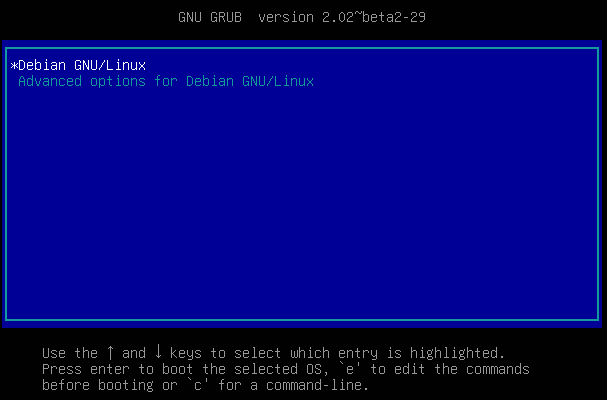
\includegraphics[width=0.9\textwidth]{grub.png}
	\caption{GRUB bootscherm}
	\label{fig:grub}
\end{figure}

Onder aan het scherm zie je hoe je GRUB kan bedienen (met de pijltjes toetsen) en dat het met e de opdracht regel kan editten (wijzigen). Dit laatste zal je niet vaak nodig hebben, maar weet dat het kan.

